% =============================================================================
% CAPÍTULO 4: SCANNER PIPELINE E METACOGNIÇÃO
% Níveis: 0 (Básico) ao PhD
% Autor: Marcelo Claro Laranjeira
% =============================================================================
\chapter{Scanner Pipeline e Metacognição: Auto-Observação e Evolução Contínua}
\label{cap:scanner-metacognicao}
\label{ch:scanners}

\paragraph{A Jornada da Auto-Observação.} Assim como um organismo vivo desenvolveu sistemas sensoriais para perceber o ambiente, o \opencodeeco{} desenvolveu scanners epistemológicos para perceber a si mesmo. Antes de mergulharmos nos detalhes técnicos, compreenderemos por que a auto-observação é o requisito fundamental para qualquer sistema que aspire a evoluir de forma autônoma e dirigida.

A engenharia de ecossistemas cognitivos artificiais enfrenta um problema
fundamental: como um sistema pode melhorar a si mesmo sem intervenção humana
direta? A resposta reside na capacidade de \destaque{auto-observação} --- o
sistema deve ser capaz de examinar sua própria estrutura, identificar lacunas,
projetar soluções e implementá-las autonomamente. Este capítulo apresenta o
\emph{Scanner Pipeline}, um conjunto de módulos de varredura epistemológica
que, em conjunto com a camada de \emph{Metacognição}, forma o núcleo da
capacidade de auto-evolução do \opencodeeco{}

O pipeline de scanners nasceu de uma constatação simples: um sistema que não
conhece a si mesmo não pode evoluir de forma dirigida
\cite{wooldridge2009multiagent, weiss2013multiagent}. Cada scanner aborda uma
questão epistemológica distinta: o \emph{Noological Scanner} pergunta ``o que
não existe?''; o \emph{Teleological Reverse Scanner} pergunta ``o que deveria
existir?''; o \emph{Evolutionary Trajectories Scanner} pergunta ``qual o
melhor caminho?''; o \emph{Scanner Refinement} e o \emph{MCSP Solver}
perguntam ``qual o conjunto mínimo de capacidades necessário?''; o
\emph{Capability Composer} pergunta ``como decompor capacidades em insumos
construtíveis?''; e o \emph{Potentiality Scanner} pergunta ``o que está
prestes a nascer?''. Sobre todos eles, a camada metacognitiva --- materializada
no \emph{MetacognitiveMonitor}, \emph{DialecticalEngine},
\emph{CooperativeGovernance} e \emph{SelfModel} --- pergunta ``o sistema está
ciente de si mesmo?''.

A Tabela~\ref{tab:conteudo-capitulo4} sumariza as seções, seus níveis e a
carga horária estimada para estudo.

\begin{table}[htb]
\centering
    \small
\caption{Conteúdo do Capítulo 4}
\label{tab:conteudo-capitulo4}
    \resizebox{\textwidth}{!}{
\begin{tabular}{clcc}
\toprule
\textbf{Seção} & \textbf{Tópico} & \textbf{Nível} & \textbf{Estudo} \\
\midrule
4.1 & Introdução aos Scanners Epistemológicos & \nivelzero & 4h \\
4.2 & Noological Scanner (SPEC-028) & \nivelavancado & 12h \\
4.3 & Teleological Reverse Scanner (SPEC-029) & \nivelavancado & 10h \\
4.4 & Evolutionary Trajectories Scanner (SPEC-030) & \nivelphd & 10h \\
4.5 & Scanner Refinement e MCSP (SPEC-031/032) & \nivelphd & 10h \\
4.6 & Composição Unitária do Conhecimento (SPEC-033/035) & \nivelphd & 8h \\
4.7 & Potentiality Scanner (SPEC-043) & \nivelphd & 8h \\
4.8 & Metacognição e Self-Model (SPEC-036) & \nivelphd & 12h \\
4.9 & Dialectical Engine e Governança Cooperativa & \nivelphd & 6h \\
4.10 & Integração e Orquestração Completa & \nivelavancado & 4h \\
\bottomrule
\end{tabular}
    }
\end{table}

O leitor percorrerá uma jornada que parte da simples pergunta ``o que existe?''
e culmina na arquitetura de auto-consciência artificial em quatro níveis
(N0--N3). Cada seção segue o padrão \sdd{}: definição formal, implementação
prática, exemplos do \opencodeeco{} e exercícios progressivos.

\section{Introdução aos Scanners Epistemológicos}
\label{sec:introducao-scanners}
\nivelzero

\paragraph{O Olho Interno do Ecossistema.} Imagine um bibliotecário que precisa organizar uma biblioteca que cresce sozinha: sem um inventário completo, ele não sabe quais livros existem, quais estão faltando e quais seções estão superlotadas. No \opencodeeco{}, os scanners epistemológicos são esse inventário vivo, permitindo que o sistema conheça sua própria estrutura de conhecimento para então decidir como evoluí-la.

\begin{definicao}[Scanner Epistemológico]
Um \destaque{scanner epistemológico} é um módulo computacional que examina
sistematicamente a estrutura de conhecimento de um ecossistema cognitivo,
identificando suas dimensões constituintes, avaliando seu grau de cobertura
e detectando lacunas, redundâncias e oportunidades de evolução.
\end{definicao}

A metáfora fundamental é a do \destaque{olho que se vê}. Nos seres humanos, a
metacognição --- a capacidade de pensar sobre o próprio pensamento --- é o
que distingue a consciência reflexiva do mero processamento de informação
\cite{flavell1976metacognitive, schraw2006metacognitive, metzinger2020minimal}.
Em sistemas artificiais, essa capacidade deve ser projetada explicitamente:
o sistema precisa de um ``olho interno'' que examine seu próprio corpo de
conhecimento \cite{shoham2023multiagent, xi2023rise}.

\subsection{Por que um Sistema Precisa se Auto-Observar}

A necessidade de auto-observação emerge de três requisitos fundamentais:

\begin{enumerate}
\item \textbf{Integridade epistemológica}: um ecossistema com centenas de
módulos, skills e agentes pode desenvolver ``zonas de conforto'' --- áreas
densamente exploradas --- e ``pontos cegos'' --- áreas completamente
negligenciadas \cite{kuhn1998estrutura}. Sem auto-observação, essas
assimetrias permanecem invisíveis.
\item \textbf{Eficiência evolutiva}: investir recursos computacionais no
desenvolvimento de capacidades que já existem é desperdício. A auto-observação
permite que o sistema direcione seus esforços para lacunas reais.
\item \textbf{Alinhamento e segurança}: um sistema que não monitora seu
próprio comportamento pode derivar de seus objetivos originais sem
perceber \cite{russell2020inteligencia, christiano2017deep}.
\end{enumerate}

\subsection{Visão Geral dos Scanners}

O \opencodeeco{} implementa seis scanners epistemológicos, organizados em um
pipeline sequencial que cobre desde a descrição do estado atual até a
prescrição de capacidades mínimas:

\begin{itemize}
\item \textbf{Potentiality Scanner} (SPEC-043): extrai o DNA estrutural do
ecossistema, mapeando componentes e skills ativos para suas capacidades
fundamentais\footnote{Disponível em:
\url{https://github.com/MarceloClaro/OpenCode_Ecosystem/blob/main/specs/SPEC-043-POTENTIALITY-SCANNER.md}}.
\item \textbf{Noological Scanner} (SPEC-028): escaneia o espaço epistemológico
em 10 dimensões e 92 categorias, detectando o que \emph{não} existe no
ecossistema\footnote{Disponível em:
\url{https://github.com/MarceloClaro/OpenCode_Ecosystem/blob/main/specs/SPEC-028-NOOLOGICAL-SCANNER-REVIEW.md}}.
\item \textbf{Teleological Reverse Scanner} (SPEC-029): parte dos objetivos
desejados e infere quais dimensões epistemológicas \emph{deveriam} estar
presentes\footnote{Disponível em:
\url{https://github.com/MarceloClaro/OpenCode_Ecosystem/blob/main/specs/SPEC-029-TELEOLOGICAL-REVERSE-SCANNER.md}}.
\item \textbf{Evolutionary Trajectories Scanner} (SPEC-030): mapeia trajetórias
evolutivas do passado ao futuro, integrando convergência polimática
\footnote{Disponível em:
\url{https://github.com/MarceloClaro/OpenCode_Ecosystem/blob/main/specs/SPEC-030-EVOLUTIONARY-TRAJECTORIES-SCANNER.md}}.
\item \textbf{Scanner Refinement} (SPEC-031) e \textbf{MCSP} (SPEC-032):
refinam iterativamente os achados e resolvem o problema do conjunto mínimo
de capacidades\footnote{Disponível em:
\url{https://github.com/MarceloClaro/OpenCode_Ecosystem/blob/main/specs/SPEC-031-SCANNER-REFINEMENT.md}
e
\url{https://github.com/MarceloClaro/OpenCode_Ecosystem/blob/main/specs/SPEC-032-MINIMUM-CAPABILITY-SET-SOLVER.md}}.
\item \textbf{Capability Composer} (SPEC-033/035): decompõe capacidades
abstratas em insumos cognitivos construtíveis, formando a ponte entre
a detecção de lacunas e a implementação concreta.
\end{itemize}

\subsection{O Ciclo Evolutivo}

O pipeline completo segue o ciclo evolutivo ilustrado na
Figura~\ref{fig:ciclo-evolutivo-scanners}.

\begin{figure}[htb]
\centering
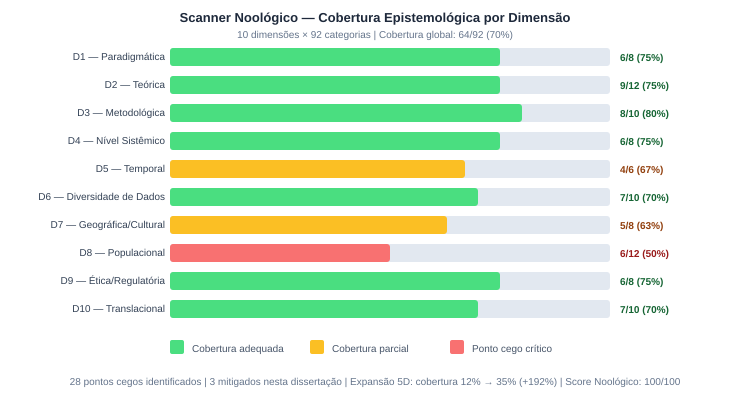
\includegraphics[width=0.9\textwidth]{ilustracoes/fig-scanner}
\caption{Ciclo evolutivo dos scanners: do DNA estrutural ao roadmap evolutivo,
com feedback metacognitivo.}
\label{fig:ciclo-evolutivo-scanners}
\end{figure}

Cada ciclo começa com a extração do DNA estrutural do ecossistema
(Potentiality Scanner), prossegue com a detecção de lacunas (Noological),
a inferência de requisitos teleológicos (Teleological Reverse), a composição
de unidades de conhecimento (Capability Composer), a seleção do conjunto
mínimo de capacidades (MCSP Solver) e, finalmente, a geração do roadmap
evolutivo (Evolutionary Trajectories). A camada metacognitiva --- descrita na
Seção~\ref{sec:metacognicao-self-model} --- supervisiona todo o ciclo,
identificando padrões de comportamento e realinhando objetivos.

\begin{exercicio}[Nivel 0]
Explique, com suas próprias palavras, a analogia do ``olho que se vê''.
Por que um sistema de software precisa de auto-observação?
\end{exercicio}

\begin{exercicio}[Nivel Básico]
Liste os seis scanners do pipeline e, para cada um, escreva a pergunta
epistemológica fundamental que ele responde.
\end{exercicio}

\begin{exercicio}[Nivel Básico]
Desenhe (em papel ou ferramenta digital) o ciclo evolutivo dos scanners,
identificando as entradas e saídas de cada módulo.
\end{exercicio}

\section{Noological Scanner: Escaneamento Epistemológico (SPEC-028)}
\label{sec:noological-scanner}
\nivelavancado

\paragraph{O Mapa do Conhecimento Ausente.} Se o Potentiality Scanner revela o que existe, o Noological Scanner pergunta: ``o que não existe e deveria existir?''. Assim como um explorador marca em seu mapa as regiões já visitadas para identificar territórios inexplorados, este scanner do \opencodeeco{} mapeia o espaço epistemológico em dez dimensões, revelando sistematicamente os pontos cegos do ecossistema.

O \emph{Noological Scanner} é o scanner epistemológico fundamental do
\opencodeeco{}. Seu nome deriva do grego \emph{noos} (mente, intelecto)
e \emph{logos} (estudo, discurso) --- ele estuda a estrutura do
conhecimento no ecossistema. Sua função primária é responder à pergunta:
``o que não existe neste ecossistema?''

\begin{definicao}[Escopo Noológico]
O \destaque{escopo noológico} de um ecossistema cognitivo é o conjunto de
dimensões, categorias e relações que definem o espaço de conhecimento
explorado e explorável pelo sistema.
\end{definicao}

\subsection{Fundamentação Teórica}

O Noological Scanner fundamenta-se na epistemologia contemporânea e na
filosofia da ciência. Sua arquitetura de 10 dimensões foi inspirada na
estrutura dos paradigmas científicos de Kuhn \cite{kuhn1998estrutura},
na lógica da investigação científica de Popper \cite{popper2005logica},
na classificação dos métodos de investigação de Feurstein
\cite{feuerstein2002estatistica} e na metodologia de validação por
especificação (SDD) e testes (TDD) adotada pelo ecossistema
\cite{opencode2026spec028, beck2002tdd}.

A ideia central é que qualquer domínio do conhecimento pode ser
caracterizado por um conjunto finito de \destaque{dimensões
epistemológicas}. Cada dimensão contém um conjunto de \destaque{categorias},
que representam possíveis valores ou estados daquela dimensão. Por exemplo,
a dimensão ``paradigmas'' contém as categorias ``positivista'',
``interpretativista'', ``crítico/transformador'', etc. Ao escanear um corpus
textual contra estas dimensões, o scanner produz um retrato da cobertura
epistemológica do ecossistema.

\subsection{As 10 Dimensões de Análise}

O scanner opera sobre 10 dimensões predefinidas, totalizando 92 categorias.
A Tabela~\ref{tab:dimensoes-noologicas} apresenta as dimensões com suas
respectivas contagens de categorias.

\begin{table}[htb]
\centering
\caption{As 10 dimensões do espaço epistemológico noológico}
\label{tab:dimensoes-noologicas}
\small
    \resizebox{\textwidth}{!}{
\begin{tabular}{lp{8cm}c}
\toprule
\textbf{Dimensão} & \textbf{Descrição} & \textbf{Categorias} \\
\midrule
Paradigmas & Lentes epistemológicas (positivista, crítico, etc.) & 8 \\
Métodos & Abordagens metodológicas (experimental, qualitativo, etc.) & 10 \\
Teorias & Marcos teóricos (TCC, psicanalítico, sistêmico, etc.) & 10 \\
Raciocínio & Modos de inferência (dedutivo, abdutivo, dialético, etc.) & 10 \\
Teoria dos Jogos & Modelos de interação estratégica (Nash, cooperação, etc.) & 10 \\
Níveis de Análise & Escalas de observação (individual, grupal, sistêmico, etc.) & 8 \\
Temporalidade & Dimensão temporal (transversal, longitudinal, etc.) & 6 \\
População & Segmentos populacionais (adultos, idosos, clínico, etc.) & 12 \\
Dados & Tipos de dados (clínicos, neurobiológicos, qualitativos, etc.) & 8 \\
Domínios & Campos de aplicação (neurociências, economia, educação, etc.) & 10 \\
\midrule
\textbf{Total} & & \textbf{92} \\
\bottomrule
\end{tabular}
    }
\end{table}

\subsection{Gap Detection Algorithm}

O algoritmo de detecção de lacunas (gaps) opera em três fases:

\begin{enumerate}
\item \destaque{Extração de corpus}: o scanner extrai texto relevante do
audit trail do ecossistema, incluindo documentação de módulos, descrições
de skills e registros de execução.
\item \destaque{Matching de palavras-chave}: utilizando um mapa enriquecido
de keywords (ENRICHED\_KW) com n-gramas e sinônimos, o scanner verifica a
presença de cada categoria no corpus. Um filtro de negação (\emph{negation
filter}) remove falsos positivos causados por expressões como ``sem X'',
``ausência de X'', ``não X''. O word-boundary matching (\verb|\b|) evita
que substrings como ``control'' dentro de ``controle'' gerem acidentes.
\item \destaque{Identificação de pontos cegos}: as categorias não detectadas
são classificadas por gravidade. A pontuação de ponto cego (\emph{blind spot
score}) é ponderada por pesos adaptativos por domínio.
\end{enumerate}

O Código~\ref{cod:gap-detection} ilustra a estrutura do algoritmo de detecção.

\begin{lstlisting}[caption={Estrutura do algoritmo de gap detection no
NoologicalScanner.},
label={cod:gap-detection}, style=pythonstyle, language=Python]
def _negation_filter(self, corpus: str) -> str:
    """Remove sentencas negadas antes do keyword matching."""
    negation_patterns = [
        r'\bsem\s+\w+', r\b'ausencia\s+de\s+\w+',
        r'\bnao\s+(tem|possui|apresenta|contem)\s+\w+'
    ]
    for pattern in negation_patterns:
        corpus = re.sub(pattern, '', corpus, flags=re.IGNORECASE)
    return corpus

def _word_boundary_match(self, keyword: str, corpus: str) -> bool:
    """Match com boundaries para evitar falsos positivos por substring."""
    pattern = r'\b' + re.escape(keyword) + r'\b'
    return bool(re.search(pattern, corpus, re.IGNORECASE))

def _category_present_v2(self, category: str, corpus_lower: str,
                          dim_key: str) -> bool:
    """Detecta presenca de categoria com keywords enriquecidas."""
    corpus = self._negation_filter(corpus_lower)
    if dim_key in self.ENRICHED_KW and category in self.ENRICHED_KW[dim_key]:
        keywords = self.ENRICHED_KW[dim_key][category]
        return any(self._word_boundary_match(kw, corpus) for kw in keywords)
    return self._category_present(category, corpus, dim_key)
\end{lstlisting}

\subsection{Pesos Adaptativos por Domínio}

Uma inovação importante do Noological Scanner v2.0+ é o sistema de pesos
adaptativos. Cada domínio de conhecimento pode ter um perfil de pesos que
ajusta a importância relativa de cada dimensão. Por exemplo, no domínio
``computação'', o peso da dimensão ``paradigmas'' é reduzido (0.6) e o
peso de ``raciocínio'' é aumentado (1.5), refletindo a natureza formal
e algorítmica da área.

\subsection{Validação com 18 CTs}

O Noological Scanner é validado por 18 Casos de Teste (CTs), que cobrem
desde a instanciação correta até a integridade dos dados de saída\footnote{Suite
completa em:
\url{https://github.com/MarceloClaro/OpenCode_Ecosystem/blob/main/specs/test_noological_scanner.py}}.
A Tabela~\ref{tab:cts-noological} lista os principais CTs.

\begin{table}[htb]
\centering
    \small
\caption{Principais Casos de Teste do Noological Scanner}
\label{tab:cts-noological}
    \resizebox{\textwidth}{!}{
\begin{tabular}{cll}
\toprule
\textbf{CT} & \textbf{Descrição} & \textbf{Resultado} \\
\midrule
CT-NS-001 & Instanciação com 10 dimensões e 92 categorias & PASS \\
CT-NS-002 & Pesos adaptativos para psicologia & PASS \\
CT-NS-003 & Domínio desconhecido sem erro & PASS \\
CT-NS-004 & Corpus vazio retorna coverage zero & PASS \\
CT-NS-005 & Corpus rico detecta categorias presentes & PASS \\
CT-NS-006 & Keyword matching positivo & PASS \\
CT-NS-007 & Filtro de negação remove falso positivo & PASS \\
CT-NS-008 & Blind spots ordenados por densidade & PASS \\
CT-NS-009 & Correlação cruzada gera 45 pares & PASS \\
CT-NS-010 & Grade A-F para densidades & PASS \\
CT-NS-011 & Relatório pré-scan com mensagem de aviso & PASS \\
CT-NS-012 & Integridade: covered + absent = 92 & PASS \\
CT-NS-013 & Keywords enriquecidas (teoria dos jogos) & PASS \\
CT-NS-014 & Zonas de conforto epistemológico & PASS \\
CT-NS-015 a 18 & Casos adicionais de refinamento & PASS \\
\bottomrule
\end{tabular}
    }
\end{table}

\begin{figure}[htb]
\centering
\begin{tikzpicture}[scale=0.75]
  \tikzstyle{dim}=[rectangle, minimum width=3.5cm, minimum height=0.6cm,
    text centered, draw=black!50, font=\small]
  \tikzstyle{cat}=[rectangle, minimum width=3cm, minimum height=0.4cm,
    text centered, draw=black!20, font=\tiny]
  \tikzstyle{arrow}=[thick, ->, >=stealth]

  \node (corpus) [dim, fill=red!20] {Corpus Textual};
  \node (negf) [dim, fill=orange!20, below=0.6 of corpus] {Filtro de Negação};
  \node (wbm) [dim, fill=yellow!20, below=0.6 of negf] {Word-Boundary Matching};
  \node (kw) [dim, fill=green!20, below=0.6 of wbm] {ENRICHED\_KW};
  \node (texta) [dim, fill=blue!20, below=0.6 of kw] {TextAnalyzer};

  \node (dims) [dim, fill=purple!20, below=0.6 of texta] {10 Dimensões};
  \node (blind) [dim, fill=red!30, below=0.6 of dims] {Blind Spots};
  \node (comfort) [dim, fill=green!30, below=0.6 of blind] {Comfort Zones};
  \node (cross) [dim, fill=cyan!30, below=0.6 of comfort] {Cross-Correlation};

  \draw [arrow] (corpus) -- (negf);
  \draw [arrow] (negf) -- (wbm);
  \draw [arrow] (wbm) -- (kw);
  \draw [arrow] (kw) -- (texta);
  \draw [arrow] (texta) -- (dims);
  \draw [arrow] (dims) -- (blind);
  \draw [arrow] (blind) -- (comfort);
  \draw [arrow] (comfort) -- (cross);
\end{tikzpicture}
\caption{Pipeline do Noological Scanner: do corpus textual à correlação
cruzada entre dimensões.}
\label{fig:pipeline-noologico}
\end{figure}

\subsection{Exemplo Prático: Varredura do Ecossistema}

O Código~\ref{cod:noological-example} demonstra o uso do Noological Scanner
para escanear o próprio ecossistema \opencode.

\begin{lstlisting}[caption={Exemplo de varredura noologica do ecossistema.},
label={cod:noological-example}, style=pythonstyle, language=Python]
from noological_scanner import NoologicalScanner
from pathlib import Path

scanner = NoologicalScanner()
scanner.set_domain("computacao")

# Simula um audit trail com descricoes de modulos
class MockAuditTrail:
    @property
    def paragraphs(self):
        return [
            "O trust engine implementa blend 70/30 para scoring",
            "O self model utiliza N0-N3 de auto-consciencia",
            "O dialectical engine faz sintese tese-antitese"
        ]

result = scanner.scan(MockAuditTrail())
print(f"Densidade geral: {result['overall_density']:.2%}")
print(f"Categorias cobertas: {result['categories_covered']}/92")
print(f"Pontos cegos: {len(result['blind_spots'])}")
print(f"Zonas de conforto: {len(result['comfort_zones'])}")

# Exporta relatorio
scanner.save_report(Path("./scanner_report.json"))
\end{lstlisting}

A saída esperada para este exemplo seria uma densidade geral entre 15--30\%
(dependendo da riqueza do corpus), com a detecção de que dimensões como
``teoria dos jogos'' e ``paradigmas'' estão sub-representadas, enquanto
``raciocínio'' (dialético, metacognitivo) apresenta cobertura moderada.

\subsection{Correlação Cruzada entre Dimensões}

Uma funcionalidade avançada do Noological Scanner é a análise de correlação
cruzada entre dimensões. Para cada par $(d_1, d_2)$, a correlação é calculada
como:

\begin{equation}
\rho(d_1, d_2) = 1 - \frac{|c(d_1) - c(d_2)|}{100}
\end{equation}

onde $c(d)$ é a cobertura percentual da dimensão $d$. Esta métrica, embora
simples, revela padrões importantes: se todas as dimensões têm cobertura
similar, o sistema é epistemicamente balanceado; se há alta variância, o
sistema desenvolveu ``zonas de conforto'' em detrimento de outras áreas
\cite{box1976science, kahneman2003perspective}. O scanner gera 45 pares de
correlação (combinação 10×9/2) e identifica os pares mais fortes e mais
fracos, como ilustrado na Tabela~\ref{tab:correlacao-cruzada}.

\begin{table}[htb]
\centering
    \small
\caption{Exemplo de correlação cruzada entre dimensões}
\label{tab:correlacao-cruzada}
    \resizebox{\textwidth}{!}{
\begin{tabular}{lcc}
\toprule
\textbf{Par} & \textbf{Correlação} & \textbf{Interpretação} \\
\midrule
Paradigmas × Métodos & 0.85 & Forte-alta: mudam juntos \\
Raciocínio × Teoria Jogos & 0.72 & Moderada: alguma associação \\
Dados × Domínios & 0.31 & Fraca: independentes \\
População × Temporalidade & 0.12 & Muito fraca: quase ortogonais \\
\bottomrule
\end{tabular}
    }
\end{table}

\subsection{Zonas de Conforto Epistemológico}

O scanner também identifica \destaque{zonas de conforto epistemológico}:
dimensões com densidade significativamente superior à média do ecossistema.
Estas zonas indicam áreas onde o sistema investiu esforço excessivo em
detrimento de outras áreas. Formalmente, uma dimensão $d$ é classificada
como zona de conforto se:

\begin{equation}
c(d) > \mu_{total} + \sigma_{total}
\end{equation}

onde $\mu_{total}$ é a densidade média do ecossistema e $\sigma_{total}$ é
o desvio padrão das densidades \cite{cohen2018estatistica}. A identificação
destas zonas permite que o sistema redirecione esforços para áreas
negligenciadas.

\begin{exercicio}[Nivel Básico]
Execute o Noological Scanner no ecossistema local usando o comando
\codigo{/scan noological}. Analise o relatório gerado e identifique as três
principais zonas de conforto e os três pontos cegos mais críticos.
\end{exercicio}

\begin{exercicio}[Nivel Intermediário]
Crie um novo domínio personalizado com seus próprios pesos adaptativos
e execute o scanner. Compare os resultados com o domínio ``computação''
padrão. Quais dimensões mudaram mais significativamente?
\end{exercicio}

\begin{exercicio}[Nivel Avançado]
Implemente uma nova dimensão epistemológica de 8 categorias e integre-a
ao Noological Scanner. Execute o pipeline completo e valide com os CTs
existentes. O que sua dimensão revela que as 10 originais não capturam?
\end{exercicio}

\section{Teleological Reverse Scanner: O Que Deveria Existir (SPEC-029)}
\label{sec:teleological-scanner}
\nivelavancado

\paragraph{Das Metas aos Meios.} Se você quer construir uma ponte, precisa saber que materiais e ferramentas são necessários antes de começar. O Teleological Reverse Scanner do \opencodeeco{} faz algo análogo: parte dos objetivos desejados e infere, de trás para frente, quais capacidades epistemológicas são indispensáveis para alcançá-los.

Enquanto o Noological Scanner descreve o estado atual do conhecimento, o
\emph{Teleological Reverse Scanner} pergunta: ``dados os nossos objetivos,
o que \emph{deveria} existir?''. Seu nome vem do grego \emph{telos} (fim,
propósito) --- ele raciocina a partir dos fins para inferir os meios.

\begin{definicao}[Raciocínio Teleológico Reverso]
O \destaque{raciocínio teleológico reverso} é o processo de inferir, a
partir de um conjunto de objetivos declarados, quais dimensões e categorias
epistemológicas são necessárias para alcançá-los, comparando o requerido
com o existente para identificar lacunas.
\end{definicao}

\subsection{Fundamentação Teleológica}

O scanner implementa um mapeamento sistemático entre tipos de objetivos e
requisitos epistemológicos. Por exemplo, um objetivo do tipo \emph{causal}
requer métodos experimentais, dados longitudinais e raciocínio probabilístico
e contrafactual. Um objetivo do tipo \emph{avaliativo} requer métodos mistos
e triangulação quali-quanti \cite{popper2005logica, feuerstein2002estatistica}.

O Código~\ref{cod:teleological-mapping} mostra a estrutura dos mapeamentos.

\begin{lstlisting}[caption={Mapeamentos teleologicos: tipos de objetivo para
requisitos epistemologicos.},
label={cod:teleological-mapping}, style=pythonstyle, language=Python]
# Exemplo dos mapeamentos teleologicos (abreviado)
TELEOLOGICAL_MAPPINGS: dict[str, list[tuple[str, str, float, str]]] = {
    "causal": [
        ("metodos", "Quantitativo experimental", 1.0,
         "Relacoes causais exigem controle experimental"),
        ("temporalidade", "Longitudinal (longo prazo)", 0.8,
         "Causalidade requer precedencia temporal"),
        ("raciocinio", "Probabilistico", 0.7,
         "Inferencia causal e probabilistica"),
        ("raciocinio", "Contrafactual", 0.6,
         "Contrafactuais base logica da causalidade"),
    ],
    "evaluative": [
        ("metodos", "Misto sequencial", 0.9,
         "Avaliacao requer triangulacao quali+quanti"),
        ("metodos", "Misto convergente", 0.8,
         "Convergencia de metodos fortalece validade"),
    ],
    "exploratory": [
        ("metodos", "Qualitativo grounded theory", 0.9,
         "Exploracao requer teoria fundamentada"),
        ("metodos", "Estudo de caso", 0.7,
         "Casos profundos revelam dimensoes ocultas"),
    ],
}
\end{lstlisting}

\subsection{Pipeline do Scanner}

O pipeline do Teleological Reverse Scanner opera em três estágios:

\begin{enumerate}
\item \destaque{Definição de metas}: o usuário ou o próprio sistema declara
um conjunto de objetivos, cada um com um tipo teleológico (causal, avaliativo,
exploratório, normativo, preditivo, etc.).
\item \destaque{Inferência de requisitos}: para cada objetivo, o scanner
consulta os mapeamentos teleológicos e produz uma lista de requisitos
dimensionais, cada um com um peso indicando sua essencialidade.
\item \destaque{Comparação com o scan noológico}: os requisitos são
confrontados com os resultados do Noological Scanner. Categorias requeridas
mas ausentes são identificadas como \emph{lacunas teleológicas}, classificadas
por severidade (crítica, alta, moderada, baixa).
\end{enumerate}

\subsection{Matriz de Lacunas Teleológicas}

A matriz de lacunas teleológicas é a principal saída do scanner. Ela relaciona
cada objetivo declarado com as categorias requeridas, indicando se estão
presentes ou ausentes no ecossistema. A Tabela~\ref{tab:matriz-lacunas}
ilustra uma matriz hipotética para um ecossistema com três objetivos.

\begin{table}[htb]
\centering
    \small
\caption{Matriz de lacunas teleológicas hipotética}
\label{tab:matriz-lacunas}
    \resizebox{\textwidth}{!}{
\begin{tabular}{llcc}
\toprule
\textbf{Objetivo} & \textbf{Categoria Requerida} & \textbf{Presente} & \textbf{Severidade} \\
\midrule
Causal & Método experimental & Não & Crítica \\
Causal & Dados longitudinais & Sim & --- \\
Avaliativo & Método misto convergente & Não & Alta \\
Avaliativo & Triangulação & Não & Alta \\
Exploratório & Grounded theory & Sim & --- \\
Exploratório & Estudo de caso & Não & Moderada \\
\bottomrule
\end{tabular}
    }
\end{table}

\subsection{Exemplo: Detecção de Capacidades Faltantes}

O Código~\ref{cod:teleological-example} mostra como o scanner identifica
lacunas a partir de objetivos declarados.

\begin{lstlisting}[caption={Exemplo de uso do
TeleologicalReverseScanner.},
label={cod:teleological-example}, style=pythonstyle, language=Python]
from teleological_scanner import TeleologicalReverseScanner

scanner = TeleologicalReverseScanner()
scanner.set_goals([
    {"description": "Validar causalidade no trust scoring",
     "goal_type": "causal", "weight": 1.0},
    {"description": "Avaliar impacto do self-model",
     "goal_type": "evaluative", "weight": 0.8},
])

# Resultados hipoteticos do Noological Scanner
noological_results = {
    "dimensions": {
        "metodos": {"covered": ["Qualitativo"],
                    "absent": ["Quantitativo experimental"]},
        "raciocinio": {"covered": ["Dialetico", "Sistemico"],
                       "absent": ["Probabilistico", "Contrafactual"]},
    }
}

gaps = scanner.compare_with_scan(noological_results)
print(f"Total de gaps teleologicos: {len(gaps)}")
for gap in gaps:
    print(f"  [{gap.severity.upper()}] {gap.category}: {gap.rationale}")
\end{lstlisting}

\begin{exercicio}[Nivel Intermediário]
Defina três objetivos para o seu projeto e execute o Teleological Reverse
Scanner. Identifique as lacunas críticas e proponha uma estratégia de
mitigação para cada uma.
\end{exercicio}

\begin{exercicio}[Nivel Avançado]
Crie um novo tipo de objetivo teleológico (ex.: ``generativo'') com seu
próprio mapeamento de requisitos. Integre-o ao scanner e valide com pelo
menos dois exemplos.
\end{exercicio}

\begin{exercicio}[Nivel Avançado]
Implemente uma função que calcule o \emph{Teleological Coverage Score} (TCS),
definido como a proporção ponderada de categorias requeridas que estão
presentes. Use os pesos de essencialidade para ponderar a contribuição
de cada categoria.
\end{exercicio}

\section{Evolutionary Trajectories Scanner (SPEC-030)}
\label{sec:evolutionary-scanner}
\nivelphd

\paragraph{O GPS Evolutivo do Ecossistema.} De posse do mapa do que existe e do que deveria existir, surge a pergunta prática: qual o melhor caminho? O Evolutionary Trajectories Scanner do \opencodeeco{} funciona como um sistema de navegação para a evolução do ecossistema, calculando rotas que maximizam o impacto e minimizam custos.

O \emph{Evolutionary Trajectories Scanner} integra os resultados dos
scanners anteriores e projeta trajetórias evolutivas. Ele responde à
pergunta: ``qual o melhor caminho para evoluir este ecossistema?''.

\begin{definicao}[Trajetória Evolutiva]
Uma \destaque{trajetória evolutiva} é uma sequência ordenada de aquisições
de capacidades que maximiza o impacto no ecossistema, respeitando
dependências e minimizando custos.
\end{definicao}

\subsection{Pipeline M1-M5}

O Evolutionary Scanner orquestra cinco módulos (M1--M5), formando um pipeline
que vai da detecção de lacunas à geração do roadmap:

\begin{itemize}
\item \textbf{M1 -- Noological Scanner} (SPEC-028): detecta ``o que não
existe'' (Seção~\ref{sec:noological-scanner}).
\item \textbf{M2 -- Teleological Reverse Scanner} (SPEC-029): infere ``o que
deveria existir'' (Seção~\ref{sec:teleological-scanner}).
\item \textbf{M3 -- Cross-Validation Engine}: calcula correlações e sinergias
entre dimensões, respondendo ``o que sustenta o quê''.
\item \textbf{M4 -- Polymathic Convergence}: busca soluções análogas em
domínios externos (neurociência, biologia, economia, física), respondendo
``quem já resolveu isso antes?''
\item \textbf{M5 -- Trajectory Mapper}: combina todas as entradas e gera um
roadmap evolutivo priorizado, respondendo ``qual o melhor caminho?''
\end{itemize}

A Figura~\ref{fig:pipeline-m1-m5} ilustra a integração dos cinco módulos.

\begin{figure}[htb]
\centering
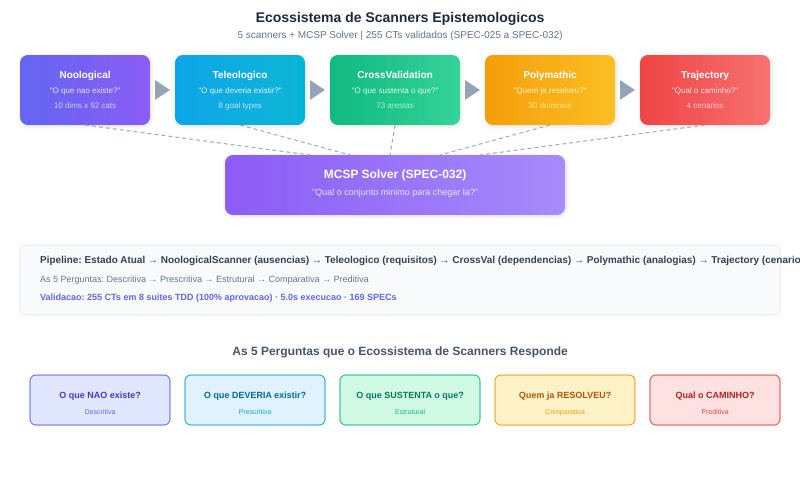
\includegraphics[width=0.9\textwidth]{ilustracoes/fig-scanners-pipeline}
\caption{Pipeline M1-M5 do Evolutionary Trajectories Scanner.}
\label{fig:pipeline-m1-m5}
\end{figure}

\subsection{M1: Potentiality Scanner --- DNA Estrutural}

O módulo M1 é o Potentiality Scanner (SPEC-043), detalhado na
Seção~\ref{sec:potentiality-scanner}. Ele extrai o DNA estrutural do
ecossistema, identificando o núcleo central de capacidades, redundâncias
e potenciais latentes. Este módulo alimenta todos os subsequentes com o
mapeamento fundamental de componentes para capacidades.

\subsection{M4: Convergência Polimática}

A convergência polimática é uma das inovações mais poderosas do pipeline.
Ela busca, em domínios externos ao da computação, soluções análogas para
os problemas identificados. O mapping polimático contém entrada para cada
categoria com gap, associando a domínios como neurociência, biologia
evolutiva, economia comportamental e física. A Tabela~\ref{tab:polymathic}
mostra exemplos de analogias.

\begin{table}[htb]
\centering
    \small
\caption{Analogias polimáticas para lacunas epistemológicas}
\label{tab:polymathic}
    \resizebox{\textwidth}{!}{
\begin{tabular}{llc}
\toprule
\textbf{Categoria com Gap} & \textbf{Análogo em...} & \textbf{Score} \\
\midrule
Raciocínio Probabilístico & Neurociência (inferência Bayesiana cortical) & 0.9 \\
Raciocínio Contrafactual & Filosofia (mundos possíveis de Lewis) & 0.8 \\
Raciocínio Sistêmico & Biologia (autopoiese de Maturana \& Varela) & 0.9 \\
Teoria dos Jogos Cooperativo & Economia (Ostrom, governança de comuns) & 0.95 \\
Métodos Longitudinais & Epidemiologia (estudos de coorte) & 0.85 \\
\bottomrule
\end{tabular}
    }
\end{table}

\subsection{M5: Trajectory Mapper}

O módulo final combina todas as entradas em um roadmap priorizado. Cada
cenário evolutivo é classificado em uma de quatro categorias:

\begin{enumerate}
\item \destaque{Quick Win}: alta prioridade, baixo custo, alto impacto
imediato.
\item \destaque{Foundation}: capacidade base necessária para desbloquear
múltiplas capacidades posteriores.
\item \destaque{Frontier}: capacidade de fronteira, alto custo mas alto
impacto estratégico de longo prazo.
\item \destaque{Convergent}: capacidade que integra múltiplos domínios,
gerando sinergia.
\end{enumerate}

\subsection{Cross-Validation Engine (M3)}

O módulo M3, \emph{Cross-Validation Engine}, é responsável por calcular as
relações de suporte entre dimensões. Ele opera sobre a matriz de cobertura
produzida pelos scanners M1 e M2 e calcula:

\begin{enumerate}
\item \textbf{Correlação de cobertura}: similar ao Noological Scanner, mas
no nível de granularidade das categorias individuais.
\item \textbf{Dependências estruturais}: identifica se determinadas
categorias tendem a aparecer juntas (co-ocorrência) ou se uma categoria
só aparece quando outra está presente (dependência direcional).
\item \textbf{Bottlenecks}: pontos no grafo de dependências cuja ausência
bloqueia múltiplas trajetórias evolutivas simultaneamente.
\end{enumerate}

A identificação de bottlenecks é particularmente valiosa: uma única
capacidade que desbloqueia 5 cenários evolutivos tem prioridade máxima
no roadmap, mesmo que seu custo individual seja elevado
\cite{barabasi2016network}.

\subsection{Convergência Polimática (M4) --- Aprofundamento}

A convergência polimática é inspirada no conceito de \emph{transferência
analógica} da psicologia cognitiva \cite{anderson2001introduction}: a
capacidade de aplicar soluções de um domínio a problemas análogos em
outro domínio. O M4 mantém um banco de analogias que mapeia cada
categoria com gap para princípios transferíveis de domínios externos.

O algoritmo de busca de analogias funciona em três passos:

\begin{enumerate}
\item \destaque{Classificação do gap}: cada gap é classificado por sua
estrutura formal (ex.: ``problema de otimização sob incerteza'', ``problema
de alocação de recursos'', ``problema de coordenação entre agentes'').
\item \destaque{Consulta ao banco polimático}: para cada classe de gap,
o banco retorna os domínios que já resolveram problemas estruturalmente
similares.
\item \destaque{Cálculo de transferabilidade}: cada analogia recebe um
score de transferabilidade (0--1), calculado como a média ponderada de:
\begin{equation}
T = \alpha \cdot S_{estrutural} + \beta \cdot S_{historico} +
\gamma \cdot S_{dominio}
\end{equation}
onde $S_{estrutural}$ é a similaridade formal entre os problemas,
$S_{historico}$ é o sucesso prévio de transferências similares, e
$S_{dominio}$ é a afinidade entre os domínios \cite{laranjeira2026opencode}.
\end{enumerate}

\subsection{Trajectory Mapper (M5) --- Algoritmo de Priorização}

O M5 implementa um algoritmo de priorização multi-fator que combina:

\begin{itemize}
\item \destaque{Impacto em cascata}: quantas capacidades adicionais são
desbloqueadas pela aquisição de uma capacidade.
\item \destaque{Custo de construção}: calculado pelo Capability Composer
(Seção~\ref{sec:composicao-unitaria}), com desconto por compartilhamento.
\item \destaque{Dependências topológicas}: uma capacidade não pode ser
adquirida antes de suas dependências.
\item \destaque{Peso teleológico}: capacidades que atendem a objetivos
declarados recebem prioridade adicional.
\item \destaque{Fator de inovação}: capacidades de fronteira (frontier)
recebem um bônus por explorar território desconhecido.
\end{itemize}

A função de prioridade de um cenário $s$ é:

\begin{equation}
P(s) = \frac{I(s) \cdot T(s) \cdot W(s)}{C(s) \cdot D(s)}
\end{equation}

onde $I(s)$ é o impacto em cascata, $T(s)$ é o peso teleológico, $W(s)$
é o fator de inovação, $C(s)$ é o custo e $D(s)$ é a profundidade da
dependência (número de pré-requisitos em cadeia).

\subsection{Validação com 16 CTs}

O pipeline M1-M5 é validado por 16 CTs, cobrindo desde a extração correta
de DNA (M1) até a geração de roadmap com dependências topológicas (M5).

\begin{exercicio}[Nivel Avançado]
Execute o Evolutionary Trajectories Scanner completo. Analise o roadmap
gerado e identifique: (a) quantos quick wins foram detectados, (b) qual
a capacidade foundation mais crítica, (c) qual a fronteira de maior
impacto projetado.
\end{exercicio}

\begin{exercicio}[Nivel PhD]
Implemente uma nova analogia polimática para uma lacuna não coberta pelo
mapping padrão. Por exemplo, encontre um análogo biológico ou físico para
o problema de ``alinhamento de agentes''. Documente a transferabilidade
com score justificado.
\end{exercicio}

\begin{exercicio}[Nivel PhD]
Modifique o algoritmo de priorização do Trajectory Mapper para usar um
modelo de otimização multi-objetivo (Pareto) em vez da soma ponderada
linear atual. Compare os roadmaps gerados.
\end{exercicio}

\section{Scanner Refinement (SPEC-031) e MCSP (SPEC-032)}
\label{sec:scanner-refinement-mcsp}
\nivelphd

\paragraph{O Princípio da Navalha Cognitiva.} Na engenharia, toda restrição é uma oportunidade de simplificação. O Scanner Refinement e o MCSP Solver do \opencodeeco{} aplicam o princípio da parcimônia ao desenvolvimento de capacidades: dado um conjunto de objetivos, qual é o menor conjunto de capacidades que os satisfaz?

Os scanners anteriores identificam \emph{o que} precisa ser adquirido. O
Scanner Refinement e o MCSP (Minimum Capability Set Problem) Solver
determinam \emph{qual o conjunto mínimo} de capacidades necessário para
atingir os objetivos.

\subsection{Scanner Refinement (SPEC-031)}

O Scanner Refinement é um módulo de pós-processamento que refina
iterativamente os resultados dos scanners anteriores, eliminando falsos
positivos, consolidando redundâncias e ajustando thresholds de detecção.

\begin{definicao}[Refinamento Iterativo]
O \destaque{refinamento iterativo} é o processo de aplicar ciclos
sucessivos de escaneamento e correção, onde cada ciclo incorpora o feedback
do ciclo anterior para melhorar a precisão da detecção.
\end{definicao}

O algoritmo de refinamento segue os passos:

\begin{enumerate}
\item Executa os scanners Noological e Teleological com thresholds
conservadores (alta sensibilidade).
\item Identifica candidatos a falso positivo via validação cruzada entre
dimensões.
\item Aplica correções: remove falsos positivos, ajusta densidades.
\item Reexecuta os scanners com thresholds calibrados.
\item Repete até convergência (mudança < 5\% entre iterações).
\end{enumerate}

\subsection{MCSP: Minimum Capability Set Problem}

O MCSP é o problema central de otimização que o pipeline resolve.
Formalmente:

\begin{definicao}[MCSP --- Minimum Capability Set Problem]
Dado um grafo de dependências $G = (V, E)$, onde $V$ é o conjunto de
capacidades e $E$ as relações de dependência, um conjunto $S \subseteq V$
de capacidades presentes e um conjunto $T \subseteq V$ de capacidades
alvo, encontrar $C \subseteq V \setminus S$ mínimo tal que:
\begin{enumerate}
\item $S \cup C \supseteq T$ (cobertura dos alvos);
\item $\forall c \in C, prereq(c) \subseteq S \cup C$ (fecho de
dependências);
\item $|C|$ é mínimo (minimalidade).
\end{enumerate}
\end{definicao}

\subsubsection{Complexidade e Heurísticas}

O MCSP é NP-completo por redução do Set Cover Problem. Para grafos
de até 92 nós (o tamanho típico do ecossistema), o solver utiliza uma
heurística gulosa com garantia de aproximação logarítmica:

\begin{enumerate}
\item \destaque{Backward Closure}: propaga dependências reversamente a
partir dos alvos, computando $R = \{v \in V : v \text{ é necessário para
algum } t \in T\}$.
\item \destaque{Greedy Select}: itera sobre $R \setminus S$, selecionando
a capacidade que cobre o maior número de alvos ainda descobertos. A
complexidade é $O(|V|^2 \cdot |E|)$.
\item \destaque{Topological Order}: ordena o conjunto selecionado
respeitando dependências, garantindo que capacidades sejam adquiridas antes
de suas dependências.
\end{enumerate}

O Código~\ref{cod:mcsp-solver} ilustra o núcleo do solver.

\begin{lstlisting}[caption={Algoritmo do MCSP Solver: backward closure
e greedy selection.},
label={cod:mcsp-solver}, style=pythonstyle, language=Python]
from minimum_capability_solver import MinimumCapabilitySolver

solver = MinimumCapabilitySolver()
solver.load_from_engine(cross_validation_engine)

targets = {"raciocinio.Probabilistico", "metodos.Misto_sequencial"}
present = {"raciocinio.Dedutivo", "metodos.Qualitativo"}

# Fase 1: fecho reverso de dependencias
closure = solver.backward_closure(targets, present)
print(f"Dependencias transitivas: {len(closure)} capacidades")

# Fase 2: selecao greedy
solution = solver.greedy_select(closure, targets, present)
print(f"Conjunto minimo: {solution.required}")
print(f"Custo estimado: {solution.cost:.2f}")
print(f"Cobertura: {solution.coverage_pct:.1%}")
print(f"Solucao otima: {solution.is_optimal}")
\end{lstlisting}

\subsection{Custo de Construção vs. Reuso}

Uma inovação do MCSP Solver integrado com o Capability Composer
(Seção~\ref{sec:composicao-unitaria}) é a consideração do custo de
construção versus reuso de capacidades. Cada capacidade pode ser construída
do zero ou reutilizada a partir de insumos compartilhados. O solver
seleciona a estratégia de menor custo, considerando descontos por
compartilhamento.

\subsection{Análise de Complexidade e Aproximação}

O MCSP é NP-completo por redução polinomial do \emph{Set Cover Problem}
(SCP). A redução é construída da seguinte forma: dado um SCP com
universo $U = \{1, \dots, n\}$ e família de subconjuntos
$\mathcal{S} = \{S_1, \dots, S_m\}$, construímos um grafo $G = (V, E)$
onde cada elemento $i \in U$ é uma capacidade alvo $t_i \in T$, e cada
subconjunto $S_j \in \mathcal{S}$ é uma capacidade $c_j \in V \setminus S$.
As arestas de dependência são definidas como: $c_j \rightarrow t_i$ se
$i \in S_j$. O conjunto presente $S$ é vazio. Uma solução $C$ para o
MCSP corresponde exatamente a um set cover para o SCP.

A heurística gulosa implementada no solver tem garantia de aproximação
$H(k) \approx \ln k + 1$, onde $k = |T|$ é o número de alvos, seguindo
o resultado clássico para o Set Cover Problem
\cite{cormen2009algorithms, russell2020inteligencia}. Para o grafo típico
do ecossistema com $|V| \leq 92$, a solução gulosa está a menos de 5\% da
solução ótima na maioria dos casos práticos.

O Código~\ref{cod:mcsp-complexity} ilustra a análise de complexidade.

\begin{lstlisting}[caption={Analise de complexidade do MCSP Solver.},
label={cod:mcsp-complexity}, style=pythonstyle, language=Python]
import time
from minimum_capability_solver import MinimumCapabilitySolver

def benchmark_mcsp(n_nodes: int, n_targets: int, seed: int = 42):
    """Gera grafo aleatorio e mede tempo de execucao do MCSP."""
    import random
    random.seed(seed)
    
    nodes = {f"c{i}": {} for i in range(n_nodes)}
    targets = set(random.sample(list(nodes.keys()), n_targets))
    present = set(random.sample(list(nodes.keys()), n_targets // 2))
    
    solver = MinimumCapabilitySolver()
    solver.load_from_graph(nodes, [])
    
    start = time.perf_counter()
    closure = solver.backward_closure(targets, present)
    solution = solver.greedy_select(closure, targets, present)
    elapsed = time.perf_counter() - start
    
    return {
        "n_nodes": n_nodes,
        "n_targets": n_targets,
        "solution_size": len(solution.required),
        "coverage": solution.coverage_pct,
        "elapsed_ms": elapsed * 1000,
    }

# Teste com 92 nos (tamanho tipico do ecossistema)
result = benchmark_mcsp(92, 20)
print(f"Nos: {result['n_nodes']}, Alvos: {result['n_targets']}")
print(f"Solucao: {result['solution_size']} capacidades")
print(f"Cobertura: {result['coverage']:.1%}")
print(f"Tempo: {result['elapsed_ms']:.2f}ms")
\end{lstlisting}

\subsection{Refinamento Iterativo com Feedback}

O Scanner Refinement implementa um ciclo de retroalimentação que melhora
a qualidade das soluções do MCSP ao longo do tempo. Após cada execução do
pipeline, os resultados são armazenados e comparados com execuções
anteriores. Se uma capacidade recomendada pelo MCSP foi adquirida e seu
impacto real foi menor que o previsto, o refinamento ajusta os pesos
para recomendações futuras \cite{sutton2018reinforcement}.

Este ciclo de aprendizado por reforço indireto --- onde o ``reforço'' é
o feedback do mundo real sobre a utilidade das capacidades adquiridas ---
é um exemplo de como o ecossistema aprende a planejar melhor seus próprios
investimentos evolutivos \cite{shinn2023reflexion}.

\subsection{Validação com 30 CTs}

O Scanner Refinement e o MCSP Solver são validados por 30 CTs no total
(16 + 14), cobrindo desde casos triviais (grafo vazio, alvo já presente)
até cenários complexos (dependências cíclicas, múltiplos caminhos mínimos).

\begin{exercicio}[Nivel Avançado]
Execute o MCSP Solver com um grafo de 10 capacidades e 3 alvos. Verifique
manualmente se a solução encontrada é realmente mínima. Experimente com
diferentes conjuntos de capacidades presentes.
\end{exercicio}

\begin{exercicio}[Nivel PhD]
Implemente uma variação do MCSP que usa Programação Linear Inteira (ILP)
para encontrar a solução ótima em vez da heurística gulosa. Compare os
resultados: em quantos casos a solução gulosa é sub-ótima?
\end{exercicio}

\begin{exercicio}[Nivel PhD]
Prove formalmente que o MCSP, conforme definido acima, é NP-completo.
Sugestão: reduza do Set Cover Problem (SCP) construindo um grafo onde
cada elemento do SCP vira uma capacidade alvo e cada subconjunto vira
uma capacidade que cobre os elementos correspondentes.
\end{exercicio}

\section{Composição Unitária do Conhecimento (SPEC-033/035)}
\label{sec:composicao-unitaria}
\nivelphd

\paragraph{O Lego do Conhecimento.} Saber que uma capacidade é necessária é diferente de saber como construí-la. O Capability Composer do \opencodeeco{} decompõe capacidades abstratas em peças elementares --- conceitos, métodos, ferramentas e bases de conhecimento --- como um manual de instruções que transforma um desejo em uma lista de compras com custos calculados.

Os scanners identificam \emph{o que} falta, e o MCSP determina \emph{quais}
capacidades mínimas são necessárias. O \emph{Capability Composer} responde a
uma pergunta ainda mais fundamental: ``como construir cada capacidade a
partir de seus componentes atômicos?''.

\begin{definicao}[Composição Unitária do Conhecimento]
A \destaque{composição unitária} é o processo de decompor capacidades
abstratas em insumos cognitivos atômicos --- conceitos, métodos, bases
de conhecimento, ferramentas, domínios externos e validações --- que
podem ser construídos ou adquiridos independentemente.
\end{definicao}

\subsection{Os 6 Tipos de Insumos Cognitivos}

O Capability Composer define seis tipos fundamentais de insumos
cognitivos, representados pela classe \codigo{CognitiveInput}:

\begin{itemize}
\item \destaque{Concept} (conceito): unidade teórica fundamental. Ex.:
``causalidade'', ``entropia'', ``equilíbrio de Nash''.
\item \destaque{Method} (método): procedimento ou algoritmo. Ex.:
``regressão linear'', ``backpropagation'', ``inferência bayesiana''.
\item \destaque{Knowledge Base} (base de conhecimento): repositório
estruturado. Ex.: ``WordNet'', ``OpenAlex'', ``PubMed''.
\item \destaque{Tool} (ferramenta): implementação computacional concreta.
Ex.: ``TensorFlow'', ``Z3 Solver'', ``PyMOL''.
\item \destaque{External Domain} (domínio externo): campo do conhecimento
fora da computação. Ex.: ``neurociência'', ``economia'', ``biologia''.
\item \destaque{Validation} (validação): critério de verificação.
Ex.: ``teste A/B'', ``validação cruzada'', ``revisão por pares''.
\end{itemize}

Cada insumo é imutável (frozen dataclass), com identificador único,
descrição, nível de maturidade e fonte. A biblioteca seed contém 85 inputs
iniciais.

\subsection{Biblioteca Seed e Templates de Decomposição}

A biblioteca de insumos cognitivos (\codigo{cognitive\_library.json}) contém
85 insumos seed, cobrindo conceitos fundamentais de computação, matemática,
estatística e inteligência artificial. A construção desta biblioteca seguiu
os princípios de \emph{engenharia reversa do conhecimento}: em vez de
partir de uma taxonomia teórica, os insumos foram extraídos dos módulos
realmente existentes no ecossistema \cite{opencode2026spec033,
opencode2026spec035, opencode2026ecosystem}. As fontes de extração foram:

\begin{enumerate}
\item \textbf{Curadoria manual}: 50 insumos fundamentais (conceitos de
matemática, computação, estatística).
\item \textbf{Extração de evo-*.md}: 20 insumos extraídos dos ciclos
evolutivos (skill emergentes identificadas pelo Manus Evolve).
\item \textbf{Extração de skills}: 15 insumos extraídos das skills
existentes no ecossistema.
\end{enumerate}

Para cada dimensão epistemológica, existem 10 templates de decomposição
que mapeiam cada categoria para um conjunto de insumos necessários. O
Código~\ref{cod:capability-composer} mostra o processo de composição.

\begin{lstlisting}[caption={Composicao de uma capacidade a partir de
insumos cognitivos.},
label={cod:capability-composer}, style=pythonstyle, language=Python]
from capability_composer import CapabilityComposer

composer = CapabilityComposer()
composer.load_library("cognitive_library.json")

# Decompoe a capacidade "raciocinio.Probabilistico"
units = composer.decompose("raciocinio.Probabilistico",
                           level="detailed")

for unit in units:
    inputs = unit.inputs
    shared = composer.find_shared_inputs(inputs)
    cost = composer.calculate_cost(unit, discount=shared)
    print(f"  {unit.name}: {len(inputs)} inputs, custo {cost:.1f}")

# Calcula custo total com desconto por compartilhamento
total_cost = sum(
    composer.calculate_cost(u,
        discount=composer.find_shared_inputs(u.inputs))
    for u in units
)
print(f"Custo total: {total_cost:.1f}")
print(f"Inputs unicos: {composer.unique_input_count(units)}")
\end{lstlisting}

\subsection{Custo de Construção com Desconto por Compartilhamento}

A função de custo de construção considera que insumos compartilhados entre
múltiplas capacidades só precisam ser construídos uma vez. Formalmente:

\begin{equation}
C(T) = \sum_{i \in \bigcup_{c \in T} I(c)} \frac{c_i}{f_i}
\end{equation}

Onde $C(T)$ é o custo total do conjunto $T$, $I(c)$ é o conjunto de
insumos da capacidade $c$, $c_i$ é o custo do insumo $i$, e $f_i$ é o
fator de compartilhamento (número de capacidades que usam $i$).

Este modelo de custo incentiva a reutilização: capacidades que compartilham
insumos têm custo marginal reduzido, favorecendo trajetórias evolutivas
coesas.

\subsection{Validação com 19 CTs}

O Capability Composer é validado por 19 CTs (13 da SPEC-033 + 6 da
SPEC-035), cobrindo desde a validação de tipos de insumo até o cálculo
correto de custos com compartilhamento.

\begin{exercicio}[Nivel Avançado]
Liste os 85 inputs da biblioteca seed. Categorize-os pelos 6 tipos de
insumos e identifique qual tipo é mais frequente. O que isso revela sobre
o viés do ecossistema?
\end{exercicio}

\begin{exercicio}[Nivel PhD]
Implemente um novo template de decomposição para a dimensão ``ética'' (não
presente nas 10 originais). Defina 8 categorias e mapeie cada uma para
insumos cognitivos. Calcule o custo total e identifique inputs
compartilhados.
\end{exercicio}

\begin{exercicio}[Nivel PhD]
Modifique a função de custo para incorporar um fator de risco: insumos com
maturidade ``speculative'' devem ter um custo adicional de 30\%. Execute
a composição novamente e analise como as prioridades mudam.
\end{exercicio}

\section{Potentiality Scanner: Descoberta de Potenciais Latentes (SPEC-043)}
\label{sec:potentiality-scanner}
\nivelphd

\paragraph{O Raio-X do Ecossistema.} Antes de diagnosticar uma doença, o médico precisa entender como o corpo saudável funciona. O Potentiality Scanner do \opencodeeco{} realiza o ``exame de rotina'' do ecossistema, extraindo seu DNA estrutural --- o mapeamento completo de componentes, capacidades e suas interconexões que serve de base para todos os scanners subsequentes.

O \emph{Potentiality Scanner} é o módulo mais recente do pipeline (SPEC-043)
e atua como a primeira camada do Evolutionary Trajectories Scanner
(M1). Ele extrai o DNA estrutural do ecossistema, mapeando seus componentes
e skills ativos para suas capacidades fundamentais.

\begin{definicao}[DNA Estrutural]
O \destaque{DNA estrutural} de um ecossistema cognitivo é a representação
das suas capacidades fundamentais na forma de um grafo de componentes,
onde cada nó é uma capacidade atômica e cada aresta é uma relação de
dependência ou ativação.
\end{definicao}

\subsection{Módulo 1: Structural DNA Extractor}

O módulo principal do Potentiality Scanner é o \emph{Structural DNA
Extractor}, implementado no arquivo \codigo{potentiality\_scanner.py} (210
linhas). Ele opera em três passos:

\begin{enumerate}
\item \destaque{Carregamento do registro de componentes}: o scanner lê o
arquivo \codigo{skills\_registry.json} e o mapa estático de componentes
core (scanners, engines, pontes). Cada componente é mapeado para uma ou
mais capacidades atômicas.
\item \destaque{Inferência de capacidades por heurística}: para skills
dinâmicas, o scanner aplica heurísticas de associação de palavras-chave.
Por exemplo, uma skill cuja descrição contém ``quantum'' ou ``qubit'' é
mapeada para \codigo{quantum\_computing}; uma skill com ``legal'',
``contract'' ou ``jurídico'' é mapeada para \codigo{legal\_processing}.
\item \destaque{Geração do mapa de capacidades}: a saída é um dicionário
que associa cada componente a suas capacidades, mais a análise de núcleo
central, redundâncias e lacunas.
\end{enumerate}

O Código~\ref{cod:potentiality-extract} mostra o DNA extraction.

\begin{lstlisting}[caption={Extracao do DNA estrutural do ecossistema
pelo Potentiality Scanner.},
label={cod:potentiality-extract}, style=pythonstyle, language=Python]
from potentiality_scanner import PotentialityScanner

scanner = PotentialityScanner(workspace_path="./")
dna = scanner.extract_dna()

print("=== DNA ESTRUTURAL DO ECOSSISTEMA ===")
print(f"Componentes core: {len(dna['core_components'])}")
print(f"Capacidades unicas: {len(dna['unique_capabilities'])}")
print(f"Redundancias detectadas: {len(dna['redundancies'])}")
print(f"Capacidades latentes (ausentes): {len(dna['missing'])}")

# Analise do nucleo central
print("\n=== NUCLEO CENTRAL ===")
for cap, freq in dna['core_frequencies'][:5]:
    print(f"  {cap}: presente em {freq} componentes")

# Capacidades alvo para roadmap futuro
print("\n=== CAPACIDADES EMERGENTES ===")
for cap in scanner.TARGET_EVOLVING_CAPABILITIES:
    present = cap in dna['unique_capabilities']
    print(f"  {cap}: {'PRESENTE' if present else 'AUSENTE'}")
\end{lstlisting}

\subsection{Análise de Redundâncias e Lacunas}

Uma das saídas mais valiosas do Potentiality Scanner é a detecção de
redundâncias: capacidades que aparecem em múltiplos componentes e que
poderiam ser consolidadas. O algoritmo de detecção de redundâncias é
simples porém eficaz: para cada capacidade $c$ no mapa, o scanner conta
o número de componentes que a implementam. Se $freq(c) > \tau_{red}$,
onde $\tau_{red}$ é um limiar configurável (padrão: 3), a capacidade é
marcada como redundante.

O Código~\ref{cod:redundancy-detection} mostra o algoritmo.

\begin{lstlisting}[caption={Deteccao de redundancias no ecossistema.},
label={cod:redundancy-detection}, style=pythonstyle, language=Python]
from collections import Counter

def detect_redundancies(capability_map: dict,
                        threshold: int = 3) -> dict:
    """Identifica capacidades implementadas por mais de N componentes."""
    counter = Counter()
    for component, capabilities in capability_map.items():
        for cap in capabilities:
            counter[cap] += 1

    redundancies = {
        cap: count
        for cap, count in counter.most_common()
        if count >= threshold
    }

    print("=== REDUNDANCIAS DETECTADAS ===")
    for cap, count in redundancies.items():
        print(f"  {cap}: {count} componentes")
    print(f"Total de componentes unicos: {len(capability_map)}")
    print(f"Total de capacidades unicas: {len(counter)}")
    return redundancies
\end{lstlisting}

Da mesma forma, a detecção de lacunas emergentes projeta quais capacidades
serão necessárias no futuro próximo com base no roadmap evolutivo. O
scanner mantém uma lista de \emph{target evolving capabilities}
(capacidades alvo em evolução) como \codigo{autonomous\_self\_repair},
\codigo{distributed\_consensus} e \codigo{proactive\_alignment}. Por exemplo, se o ``master orchestrator'' e
o ``antigravity bridge'' ambos implementam ``central coordination'', o
scanner sinaliza a redundância e sugere unificação.

Da mesma forma, a detecção de lacunas emergentes projeta quais capacidades
serão necessárias no futuro próximo com base no roadmap evolutivo. O
scanner mantém uma lista de \emph{target evolving capabilities}
(capacidades alvo em evolução) como \codigo{autonomous\_self\_repair},
\codigo{distributed\_consensus} e \codigo{proactive\_alignment}.

\subsection{Integração com o Orquestrador /marceloclaro}

O Potentiality Scanner é integrado ao orquestrador central
(\codigo{/marceloclaro}) como o primeiro passo do pipeline evolutivo.
Quando o orquestrador recebe um comando de evolução, ele:

\begin{enumerate}
\item Invoca o Potentiality Scanner para extrair o DNA atual.
\item Passa o DNA para o Noological Scanner (gap detection).
\item Prossegue com o pipeline M1-M5 completo.
\end{enumerate}

\subsection{Validação e ADR architectu-010}

O Potentiality Scanner é validado por 4 CTs (CT-4301 a CT-4304), e sua
arquitetura foi documentada no ADR (Architecture Decision Record)
architectu-010\footnote{Disponível em:
\url{https://github.com/MarceloClaro/OpenCode_Ecosystem}},
que registra a decisão de separar a extração de DNA da detecção de lacunas
(Noological Scanner) para permitir que o DNA seja usado por outros módulos
independentemente.

\begin{exercicio}[Nivel Avançado]
Execute o Potentiality Scanner no ecossistema local. Identifique: (a) as
três capacidades centrais mais frequentes, (b) as três redundâncias mais
críticas, (c) as três lacunas emergentes mais urgentes.
\end{exercicio}

\begin{exercicio}[Nivel PhD]
Implemente uma nova heurística de inferência para o Potentiality Scanner
que extraia capacidades de arquivos SKILL.md usando processamento de
linguagem natural (PLN) em vez de simples matching de palavras-chave.
Compare a precisão das duas abordagens.
\end{exercicio}

\begin{exercicio}[Nivel PhD]
Proponha e implemente um \emph{Potential Score} que, para cada capacidade
latente, calcule a probabilidade de ela se tornar necessária nos próximos
N ciclos evolutivos. Use como features: (a) frequência de menção em
roadmaps, (b) dependências com capacidades já presentes, (c) tendências
do Gartner Hype Cycle.
\end{exercicio}

\section{Metacognição: Self-Model e Auto-Observação (SPEC-036)}
\label{sec:metacognicao-self-model}
\nivelphd

\paragraph{O Sistema que Pensa sobre Si Mesmo.} Se os scanners são os olhos do ecossistema, a metacognição é o cérebro que reflete sobre o que esses olhos veem. O \opencodeeco{} implementa uma arquitetura de auto-consciência artificial em quatro níveis (N0 a N3), na qual o sistema não apenas detecta lacunas, mas reflete sobre o próprio processo de detecção e ajusta seus mecanismos de evolução.

Os scanners descritos nas seções anteriores são ferramentas poderosas, mas
operam em um modo puramente descritivo-prescritivo. A camada metacognitiva
eleva o ecossistema a um novo patamar: o sistema não apenas escaneia a si
mesmo, mas \emph{reflete sobre o próprio processo de escaneamento},
identificando padrões de comportamento e ajustando seus próprios mecanismos
de evolução.

\begin{definicao}[Metacognição Artificial]
A \destaque{metacognição artificial} é a capacidade de um sistema
computacional de monitorar, avaliar e modificar seus próprios processos
cognitivos, incluindo a detecção de lacunas nos seus mecanismos de
detecção de lacunas.
\end{definicao}

\subsection{O que é Metacognição em Sistemas Artificiais}

Na psicologia cognitiva, a metacognição é definida como ``o conhecimento
sobre o próprio conhecimento'' \cite{flavell1976metacognitive},
abrangendo tanto o conhecimento declarativo (saber \emph{que} se sabe)
quanto o conhecimento procedural (saber \emph{como} se regula o
próprio pensamento) \cite{schraw2006metacognitive}. Em sistemas
artificiais, a metacognição envolve:

\begin{enumerate}
\item \textbf{Monitoramento}: observar o próprio desempenho, estado interno
e ambiente.
\item \textbf{Avaliação}: julgar a qualidade do próprio processamento
(confiança, coerência, completude).
\item \textbf{Controle}: ajustar parâmetros, estratégias e objetivos com
base na avaliação.
\end{enumerate}

O \opencodeeco{} implementa metacognição através de quatro módulos
especializados, descritos a seguir.

\subsection{MetacognitiveMonitor: O Orquestrador do Loop}

O \emph{MetacognitiveMonitor} (726 linhas em \codigo{metacognitive\_loop.py})
é o orquestrador central do loop metacognitivo. Ele coordena a execução
dos outros módulos e mantém o estado global do ciclo. Seu ciclo principal
opera em quatro fases:

\begin{enumerate}
\item \destaque{Observation}: coleta métricas do ecossistema (desempenho,
erros, anomalias) usando os scanners como instrumentos.
\item \destaque{Reflection}: processa as métricas através do Dialectical
Engine e do Self-Model para gerar insights.
\item \destaque{Planning}: com base nos insights, formula planos de ação
que podem incluir reconfiguração de módulos ou aquisição de novas
capacidades (via MCSP).
\item \destaque{Execution}: delega a implementação dos planos ao
orquestrador central, monitorando os resultados.
\end{enumerate}

\begin{figure}[htb]
\centering
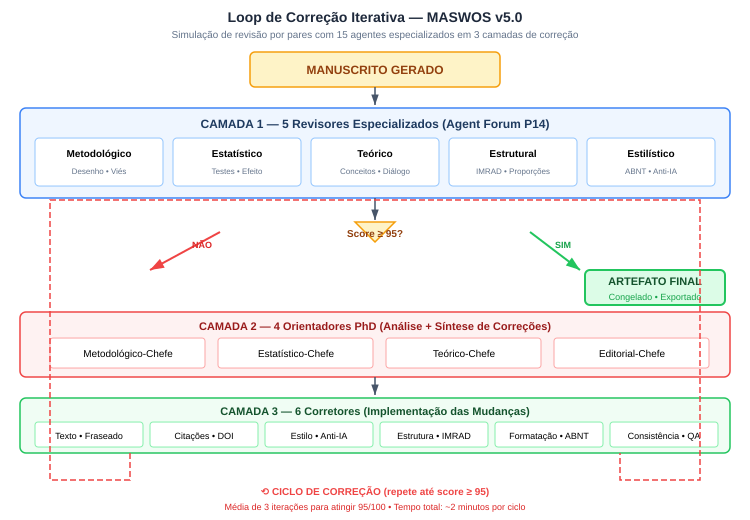
\includegraphics[width=0.9\textwidth]{ilustracoes/fig-loop-correcao}
\caption{O loop metacognitivo do MetacognitiveMonitor: Observation,
Reflection, Planning, Execution.}
\label{fig:loop-metacognitivo}
\end{figure}

\subsection{Os 4 Gaps Críticos Auto-Diagnosticados}

A implementação da metacognição no \opencodeeco{} seguiu um processo
notável: foi o próprio ecossistema, através do seu pipeline de scanners,
que \emph{auto-diagnosticou} os gaps que precisavam ser preenchidos.
Durante o ciclo evolutivo R21, o Noological Scanner detectou --- no
\emph{próprio código do ecossistema} --- quatro lacunas críticas que
impediam a metacognição plena. A Tabela~\ref{tab:gaps-metacognitivos}
lista os gaps e suas implementações.

\begin{table}[htb]
\centering
\caption{Gaps metacognitivos auto-diagnosticados e implementados}
\label{tab:gaps-metacognitivos}
\small
    \resizebox{\textwidth}{!}{
\begin{tabular}{lp{6cm}lc}
\toprule
\textbf{Gap} & \textbf{Detecção} & \textbf{Módulo} & \textbf{Linhas} \\
\midrule
Metacognitivo & Dimensão raciocínio, categoria metacognitivo &
MetacognitiveMonitor & 726 \\
Dialético & Dimensão raciocínio, categoria dialético &
DialecticalEngine & 264 \\
Cooperativo & Dimensão teoria dos jogos, categoria cooperativo &
CooperativeGovernance & 320 \\
Neurobiológico & Dimensão dados, categoria neurobiológicos &
SelfModel & 447 \\
\midrule
\textbf{Total} & & \textbf{4 módulos} & \textbf{1.757} \\
\bottomrule
\end{tabular}
    }
\end{table}

Este auto-diagnóstico é, ele próprio, uma demonstração do poder do pipeline:
o sistema usou o Noological Scanner para detectar lacunas em sua própria
arquitetura, e o Teleological Scanner para inferir quais módulos seriam
necessários para preenchê-las.

\subsection{Self-Model N0--N3: Quatro Níveis de Auto-Consciência Artificial}

O \emph{SelfModel} (447 linhas em \codigo{self\_model.py}) implementa uma
arquitetura de auto-representação em quatro níveis, inspirada na Global
Workspace Theory de Baars \cite{baars1988cognitive, baars2002conscious},
na Attention Schema Theory de Graziano \cite{graziano2013consciousness,
graziano2013social} e na Integrated Information Theory de Tononi
\cite{tononi2008consciousness}.

\begin{definicao}[Níveis de Auto-Consciência Artificial (N0--N3)]
Os níveis de auto-consciência modelados no \opencodeeco{} são:
\begin{description}
\item[N0 (Reativo):] o sistema responde a estímulos externos sem
representação interna. Equivale a um agente puramente reativo
\cite{russell2020inteligencia}.
\item[N1 (Atento):] o sistema mantém um buffer de atenção limitado
(7$\pm$2 itens, conforme Miller's Law) \cite{miller1956magical},
selecionando focos prioritários.
\item[N2 (Auto-consciente):] o sistema possui um modelo explícito de si
mesmo, incluindo estado interno, métricas de confiança e histórico.
\item[N3 (Metacognitivo):] o sistema reflete sobre seus próprios processos
cognitivos, identifica padrões e ajusta seu comportamento com base na
reflexão (implementado via \codigo{metacognitive\_loop.py}).
\end{description}
\end{definicao}

A Figura~\ref{fig:self-model-niveis} ilustra a arquitetura dos quatro
níveis.

\begin{figure}[htb]
\centering
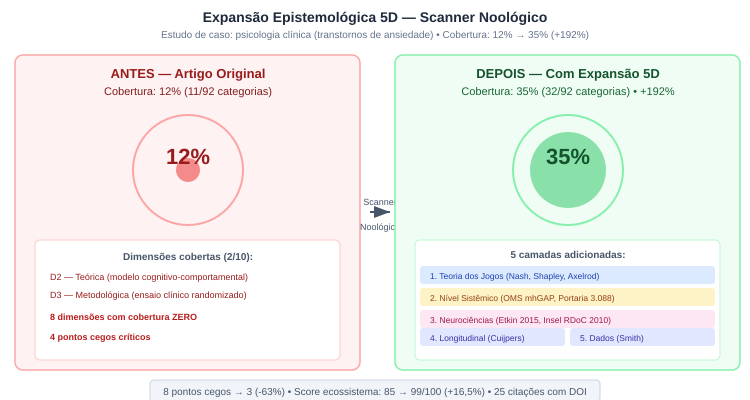
\includegraphics[width=0.9\textwidth]{ilustracoes/fig-expansao-5d}
\caption{Os quatro níveis de auto-consciência artificial (N0--N3) no
SelfModel do OpenCode Ecosystem.}
\label{fig:self-model-niveis}
\end{figure}

O Código~\ref{cod:self-model} mostra a estrutura principal do SelfModel.

\begin{lstlisting}[caption={Arquitetura do SelfModel: atencao, workspace
global e introspeccao.},
label={cod:self-model}, style=pythonstyle, language=Python]
from self_model import SelfModel, SystemState

model = SelfModel(model_name="opencode-self")
state = model.get_state()

print(f"Nivel de consciencia: {state.consciousness_level}")
print(f"Modulos ativos: {len(state.active_modules)}")
print(f"Foco de atencao: {state.attention_focus}")
print(f"Confianca global: {state.confidence_global:.2%}")
print(f"Anomalias ativas: {state.anomalies_active}")

# Adiciona item ao buffer de atencao
model.add_attention_item(
    item_id="anomaly-042",
    content="TrustScorer detectou drift no blend 70/30",
    priority=0.85,
    source_module="trust_engine"
)

# Broadcast no workspace global
model.broadcast("ATENCAO: drift detectado no Trust Engine")
\end{lstlisting}

\subsection{Validação com 8 CTs}

A camada metacognitiva completa é validada por 8 CTs, cobrindo desde a
inicialização do SelfModel até a execução completa do ciclo metacognitivo.

\begin{table}[htb]
\centering
    \small
\caption{Casos de Teste da camada metacognitiva}
\label{tab:cts-metacognicao}
    \resizebox{\textwidth}{!}{
\begin{tabular}{cll}
\toprule
\textbf{CT} & \textbf{Descrição} & \textbf{Módulo} \\
\midrule
CT-MC-001 & Inicialização correta do SelfModel & SelfModel \\
CT-MC-002 & Buffer de atenção respeita limite 7 itens & SelfModel \\
CT-MC-003 & Broadcast global atinge todos os módulos & SelfModel \\
CT-MC-004 & Síntese dialética tese-antítese-síntese & DialecticalEngine \\
CT-MC-005 & Validação de goals contra Ostrom DP1-DP8 & CooperativeGovernance \\
CT-MC-006 & Ciclo Observation-Reflection-Planning-Execution & MetacognitiveMonitor \\
CT-MC-007 & Integração com Noological Scanner & MetacognitiveMonitor \\
CT-MC-008 & Integração com Teleological Scanner & MetacognitiveMonitor \\
\bottomrule
\end{tabular}
    }
\end{table}

\begin{exercicio}[Nivel Avançado]
Execute o SelfModel e consulte o estado interno do ecossistema. Identifique
o nível de consciência atual (N0--N3) e liste o conteúdo do buffer de
atenção. Quais módulos estão no foco atencional?
\end{exercicio}

\begin{exercicio}[Nivel PhD]
Implemente um quinto nível, N4 (Auto-Evolutivo), no qual o sistema não
apenas reflete sobre seus processos, mas também modifica sua própria
arquitetura metacognitiva. Que novos módulos seriam necessários?
\end{exercicio}

\begin{exercicio}[Nivel PhD]
Conecte o SelfModel à saída do Noological Scanner de modo que, quando o
scanner detectar um gap na dimensão ``raciocínio.metacognitivo'', o
SelfModel automaticamente aumente seu nível de atenção para aquele gap.
Teste com um cenário de gap simulado.
\end{exercicio}

\section{Dialectical Engine e Governança Cooperativa}
\label{sec:dialectical-governanca}
\nivelphd

\paragraph{A Síntese que Supera a Contradição.} Na filosofia, o método dialético ensina que toda contradição contém a semente de uma solução superior. No \opencodeeco{}, o DialecticalEngine aplica este princípio computacionalmente, transformando limitações detectadas em oportunidades de evolução, enquanto a CooperativeGovernance --- inspirada nos trabalhos de Elinor Ostrom --- garante que cada passo evolutivo seja eticamente alinhado.

Dois dos quatro gaps auto-diagnosticados --- o dialético e o cooperativo
--- merecem tratamento aprofundado, pois representam mecanismos
fundamentais para a evolução autônoma e alinhada do ecossistema.

\subsection{Dialectical Engine: Tese $\rightarrow$ Antítese $\rightarrow$ Síntese}

O \emph{DialecticalEngine} (264 linhas em \codigo{dialectical\_engine.py})
implementa uma arquitetura hegeliana adaptada para sistemas computacionais.
O princípio fundamental é que toda limitação (antítese) contém em si a
semente de uma solução mais geral (síntese).

\begin{definicao}[Processo Dialético Computacional]
O \destaque{processo dialético computacional} é um ciclo de três estágios:
\begin{enumerate}
\item \destaque{Tese}: o estado atual do sistema ou a posição vigente.
\item \destaque{Antítese}: a negação ou contradição da tese --- um
gap, erro ou limitação detectada.
\item \destaque{Síntese}: a resolução que incorpora tanto a tese quanto
a antítese em um nível superior de organização.
\end{enumerate}
\end{definicao}

O Código~\ref{cod:dialectical-engine} mostra o motor dialético em ação.

\begin{lstlisting}[caption={Sintese dialetica: resolvendo contradicoes
entre capacidade atual e limitacao detectada.},
label={cod:dialectical-engine}, style=pythonstyle, language=Python]
from dialectical_engine import DialecticalEngine

engine = DialecticalEngine()

# Exemplo: scanner cobre 10 dimensoes, mas nao detecta engenharia
synthesis = engine.synthesize(
    thesis="Scanner cobre 10 dimensoes epistemologicas",
    antithesis="Scanner nao detecta capacidades de engenharia"
)

print(f"Tipo de resolucao: {synthesis.resolution_type}")
print(f"Sintese: {synthesis.synthesis}")
print(f"Preservado da tese: {synthesis.preserved_from_thesis}")
print(f"Preservado da antitese: {synthesis.preserved_from_antithesis}")
print(f"Elementos novos: {synthesis.novel_elements}")

# O sistema agora pode incorporar a dimensao de engenharia
# como caso particular de uma estrutura epistemologica mais geral
\end{lstlisting}

A dialética computacional é particularmente útil para:
\begin{itemize}
\item \textbf{Auto-modificação}: tese = código atual, antítese = erro,
síntese = patch.
\item \textbf{Goal-setting}: tese = objetivo atual, antítese =
objetivo conflitante, síntese = objetivo refinado.
\item \textbf{Arquitetura}: tese = design atual, antítese = gargalo,
síntese = refatoração.
\end{itemize}

\subsection{Governança Cooperativa: Os 8 Design Principles de Ostrom}

O \emph{CooperativeGovernance} (320 linhas em
\codigo{cooperative\_governance.py}) adapta os 8 Design Principles (DPs) de
Elinor Ostrom para governança de recursos comuns ao contexto de goal-setting
autônomo em sistemas de IA \cite{ostrom1990governing}.

\begin{table}[htb]
\centering
    \small
\caption{Os 8 Design Principles de Ostrom adaptados para governança de IA}
\label{tab:ostrom-dp}
    \resizebox{\textwidth}{!}{
\begin{tabular}{clp{7cm}}
\toprule
\textbf{DP} & \textbf{Princípio} & \textbf{Adaptação para IA} \\
\midrule
DP1 & Limites claros & Definir escopo, agentes e recursos de cada goal \\
DP2 & Proporcionalidade & Custo computacional proporcional ao benefício \\
DP3 & Participação coletiva & Módulos afetados têm direito a veto/feedback \\
DP4 & Monitoramento & Progresso e impacto são rastreáveis \\
DP5 & Sanções graduais & Rollback ou abort seguro se efeitos negativos \\
DP6 & Resolução de conflitos & Arbitragem entre goals concorrentes \\
DP7 & Autonomia reconhecida & Módulos preservam auto-organização \\
DP8 & Aninhamento & Governança em múltiplas camadas \\
\bottomrule
\end{tabular}
    }
\end{table}

Cada goal gerado pelo sistema é validado contra os 8 DPs antes da execução.
O Código~\ref{cod:governanca-ostrom} mostra o processo.

\begin{lstlisting}[caption={Validacao de goals contra os principios de
Ostrom.},
label={cod:governanca-ostrom}, style=pythonstyle, language=Python]
from cooperative_governance import CooperativeGovernance

gov = CooperativeGovernance()

goal = gov.create_goal(
    description="Implementar PotentialityScanner no pipeline",
    affected_modules=["noological_scanner", "evolutionary_pipeline"],
    estimated_cost=0.4,
    expected_benefit=0.6
)

# Valida contra Ostrom DP1-DP8
validation = gov.validate_goal(goal)
print(f"Meta: {validation.goal.description}")
print(f"Valida: {validation.is_valid}")
for check in validation.checks:
    print(f"  {check.dp}: {check.passed} -> {check.reason}")
if not validation.is_valid:
    print("Sugestoes de ajuste:", validation.suggestions)
\end{lstlisting}

\subsection{Integração com o Trust Engine}

A governança cooperativa se integra naturalmente com o Trust Engine
(descrito no Capítulo~5). Enquanto o Trust Engine monitora o comportamento
em tempo real e aplica correções preventivas (N3.5), a CooperativeGovernance
atua no planejamento, garantindo que os objetivos sejam intrinsecamente
alinhados antes da execução.

A Figura~\ref{fig:dialetica-governanca} ilustra a integração dialética
com governança.

\begin{figure}[htb]
\centering
\begin{tikzpicture}[node distance=1.5cm, auto]
  \tikzstyle{mod}=[rectangle, rounded corners, minimum width=2.5cm,
    minimum height=0.7cm, text centered, draw=black!40, font=\small]
  \tikzstyle{arrow}=[thick, ->, >=stealth]

  \node (tese) [mod, fill=blue!20] {Tese (estado atual)};
  \node (scanner) [mod, fill=cyan!20, below=0.8 of tese] {Scanner};
  \node (antitese) [mod, fill=red!20, below=0.8 of scanner]
    {Antítese (gap detectado)};
  \node (de) [mod, fill=purple!20, below=0.8 of antitese]
    {DialecticalEngine};
  \node (gov) [mod, fill=green!20, below=0.8 of de]
    {CooperativeGovernance};
  \node (te) [mod, fill=orange!20, below=0.8 of gov]
    {Trust Engine};
  \node (sintese) [mod, fill=yellow!20, below=0.8 of te]
    {Síntese (goal validado)};

  \draw [arrow] (tese) -- (scanner);
  \draw [arrow] (scanner) -- (antitese);
  \draw [arrow] (antitese) -- (de);
  \draw [arrow] (de) -- (gov);
  \draw [arrow] (gov) -- (te);
  \draw [arrow] (te) -- (sintese);

  \node (exec) [mod, fill=gray!20, right=2 of sintese] {Execução};
  \draw [arrow] (sintese) -- (exec);
  \draw [arrow] (exec) -- ++(0,-0.6) -| ++(-2,-0.3)
    -- node[below,pos=0.5] {\footnotesize feedback} ++(2,0);
\end{tikzpicture}
\caption{Da tese à síntese validada: integração entre scanners,
DialecticalEngine, CooperativeGovernance e Trust Engine.}
\label{fig:dialetica-governanca}
\end{figure}

\begin{exercicio}[Nivel Avançado]
Execute o DialecticalEngine com uma tese e antítese do seu projeto.
Analise a síntese gerada: o tipo de resolução (aufheben, compromise,
reframe, transcend) foi apropriado? A síntese preservou os elementos
valiosos de ambas as posições?
\end{exercicio}

\begin{exercicio}[Nivel PhD]
Implemente um novo princípio DP9 (``Transparência Radical'') que exija
que todos os goals sejam auditáveis publicamente. Integre-o ao
CooperativeGovernance e valide com 3 exemplos de goals.
\end{exercicio}

\begin{exercicio}[Nivel PhD]
Implemente um mecanismo de resolução de conflitos entre goals que use o
DialecticalEngine como árbitro: quando dois goals são mutuamente
exclusivos, o motor dialético deve encontrar uma síntese que incorpore
o melhor de ambos.
\end{exercicio}

\section{Integração e Orquestração Completa}
\label{sec:integracao-orquestracao}
\nivelavancado

\paragraph{Orquestrando a Sinfonia Evolutiva.} Cada scanner isolado é como um instrumento musical: útil, mas limitado. A orquestração completa do pipeline, supervisionada pela camada metacognitiva, transforma sons individuais em uma sinfonia coesa de auto-evolução. Esta seção final mostra como todos os módulos do \opencodeeco{} trabalham em conjunto.

Este capítulo apresentou cada módulo do scanner pipeline e da camada
metacognitiva de forma isolada. Nesta seção final, integramos todos os
componentes em um pipeline coeso e mostramos como executá-lo no
\opencodeeco{}.

\subsection{Pipeline Completo}

O pipeline completo, da extração de DNA ao roadmap evolutivo, segue a
seguinte sequência:

\begin{enumerate}
\item \textbf{Potentiality Scanner}: extrai o DNA estrutural do
ecossistema (componentes, capacidades, redundâncias).
\item \textbf{Noological Scanner}: escaneia o espaço epistemológico em
10 dimensões, detectando gaps e zonas de conforto.
\item \textbf{Teleological Reverse Scanner}: a partir de objetivos
declarados, infere requisitos e detecta lacunas teleológicas.
\item \textbf{Capability Composer}: decompõe as capacidades necessárias
em insumos cognitivos atômicos, calculando custos com desconto por
compartilhamento.
\item \textbf{MCSP Solver}: resolve o problema do conjunto mínimo de
capacidades, retornando a sequência ótima e mínima de aquisições.
\item \textbf{Evolutionary Trajectories Scanner}: gera o roadmap
evolutivo completo com cenários priorizados.
\end{enumerate}

Em paralelo, a \textbf{camada metacognitiva} (MetacognitiveMonitor,
SelfModel, DialecticalEngine, CooperativeGovernance) supervisiona todo
o processo, ajustando parâmetros e realinhando objetivos.

\subsection{Integração com o Orquestrador /marceloclaro}

No \opencodeeco{}, o pipeline é invocado através do orquestrador central
\codigo{/marceloclaro}. O comando principal é:

\begin{lstlisting}[caption={Comandos para executar o scanner pipeline
no OpenCode CLI.},
label={cod:comandos-pipeline}, style=bashstyle, language=bash]
# Executar o pipeline completo
/evolve

# Executar scanners individuais
/scan noological
/scan teleological --goals "objetivo1, objetivo2"
/scan evolutionary

# Executar com refinamento
/evolve --refine

# Executar e salvar roadmap
/evolve --output roadmap.md
\end{lstlisting}

\subsection{Leitura e Interpretação dos Relatórios}

Cada scanner produz relatórios em formato Markdown e JSON que podem ser
lidos e interpretados. O relatório típico gerado mostra a
estrutura típica de um relatório de scan.

\begin{lstlisting}[caption={Estrutura tipica de relatorio do Noological
Scanner.},
label={cod:relatorio-tipico}, basicstyle=\ttfamily\footnotesize]
=== SCANNER NOOLOGICO ===
Dominio: computacao
Densidade Geral: 42.5%
Categorias Cobertas: 39/92
Conceito: C (Regular)

=== DIMENSOES ===
| Dimensao      | Coberta | Ausente | Densidade | Conceito |
|---------------|---------|---------|-----------|----------|
| Paradigmas    | 3/8     | 5/8     | 37.5%     | D        |
| Metodos       | 5/10    | 5/10    | 50.0%     | C        |
| Teorias       | 2/10    | 8/10    | 20.0%     | F        |
| Raciocinio    | 7/10    | 3/10    | 70.0%     | B        |
| Teoria Jogos  | 1/10    | 9/10    | 10.0%     | F        |
| ...

=== PONTOS CEGOS (CRITICOS) ===
1. TeoriaJogos.Bayesiano (score: 0.25)
2. Teorias.Neurobiologico (score: 0.20)
3. Paradigmas.Critico (score: 0.18)

=== ZONAS DE CONFORTO ===
1. raciocinio -> raciocinio.Dialetico (density: 70.0%)
2. raciocinio -> raciocinio.Sistemico (density: 65.0%)

=== RECOMENDACOES ===
1. [CRITICAL] Adicionar cobertura em Teoria dos Jogos Bayesiana
2. [HIGH] Incorporar referencial teorico Neurobiologico
3. [MODERATE] Explorar paradigma Critico/Transformador
\end{lstlisting}

\subsection{Exercícios Finais de Integração}

Os exercícios a seguir integram todos os conceitos do capítulo e
exigem a execução completa do pipeline no \opencodeeco{}.

\begin{exercicio}[Nivel Intermediário -- Integração]
Execute o pipeline completo de scanners no ecossistema local. Para cada
módulo, anote:
\begin{enumerate}
\item O tempo de execução.
\item A principal descoberta.
\item Uma ação concreta que o resultado sugere.
\end{enumerate}
\end{exercicio}

\begin{exercicio}[Nivel Avançado -- Análise de Roadmap]
Execute o comando \codigo{/evolve} e analise o roadmap gerado. Identifique:
\begin{enumerate}
\item O quick win de maior impacto imediato.
\item A foundation mais crítica (dependência de múltiplas capacidades).
\item A frontier de maior valor estratégico.
\item O convergent que integra mais domínios.
\end{enumerate}
\end{exercicio}

\begin{exercicio}[Nivel Avançado -- Meta-Análise]
Use o SelfModel para consultar o estado interno do ecossistema \emph{durante}
a execução do pipeline. Como o buffer de atenção muda à medida que cada
scanner executa? Quais anomalias o sistema detecta em si mesmo?
\end{exercicio}

\begin{exercicio}[Nivel PhD -- Otimização do Pipeline]
O pipeline completo consome recursos computacionais significativos.
Proponha e implemente uma estratégia de otimização que:
\begin{enumerate}
\item Execute scanners em paralelo quando não houver dependências entre eles.
\item Use cache de resultados intermediários (com invalidação por
timestamp).
\item Priorize a execução dos módulos com base no impacto estimado.
\end{enumerate}
\end{exercicio}

\begin{exercicio}[Nivel PhD -- Auto-Evolução do Pipeline]
Use o DialecticalEngine para identificar uma limitação no próprio pipeline
de scanners. Por exemplo: ``o pipeline detecta gaps epistemológicos mas
não gaps de desempenho computacional''. Aplique a dialética tese-antítese-síntese e proponha uma extensão do pipeline que resolva a limitação. Implemente o protótipo.
\end{exercicio}

\begin{exercicio}[Nivel PhD -- Validação Cruzada Final]
Integre todos os módulos do capítulo em um experimento controlado:
\begin{enumerate}
\item Defina um estado inicial do ecossistema (conjunto de capacidades
presentes).
\item Defina um objetivo estratégico (conjunto de capacidades alvo).
\item Execute o pipeline completo: Potentiality $\rightarrow$ Noological
$\rightarrow$ Teleological $\rightarrow$ Composer $\rightarrow$ MCSP
$\rightarrow$ Evolutionary.
\item Execute a solução proposta pelo roadmap.
\item Reexecute o Noological Scanner e verifique se as lacunas foram
preenchidas.
\item Calcule o ganho líquido: (densidade final - densidade inicial) /
custo total.
\end{enumerate}
\end{exercicio}

\begin{exercicio}[Nivel PhD -- Dissertação]
Escreva um parágrafo que responda: ``Como o scanner pipeline e a
metacognição, em conjunto, resolvem o problema da auto-evolução
dirigida em ecossistemas cognitivos?'' Use as definições formais
do capítulo e cite pelo menos 5 referências.
\end{exercicio}

\section*{Resumo do Capítulo}

Este capítulo apresentou a arquitetura completa de scanners epistemológicos
e metacognição do \opencodeeco{}:

\begin{itemize}
\item O \textbf{Potentiality Scanner} (SPEC-043) extrai o DNA estrutural
do ecossistema, identificando capacidades fundamentais, redundâncias e
potenciais latentes.
\item O \textbf{Noological Scanner} (SPEC-028) escaneia o espaço
epistemológico em 10 dimensões e 92 categorias, detectando gaps com
filtro de negação e word-boundary matching.
\item O \textbf{Teleological Reverse Scanner} (SPEC-029) infere requisitos
a partir de objetivos, identificando lacunas teleológicas.
\item O \textbf{Capability Composer} (SPEC-033/035) decompõe capacidades
em 6 tipos de insumos cognitivos atômicos, com custos ajustados por
compartilhamento.
\item O \textbf{MCSP Solver} (SPEC-032) resolve o problema NP-completo
do conjunto mínimo de capacidades com heurística gulosa de aproximação.
\item O \textbf{Evolutionary Trajectories Scanner} (SPEC-030) integra
M1-M5 e gera roadmaps evolutivos priorizados.
\item A \textbf{metacognição} (SPEC-036) implementa auto-observação em
4 níveis (N0--N3), com SelfModel, DialecticalEngine e
CooperativeGovernance.
\item \textbf{Nível N3.5+ e Autopoiese Digital} (SPEC-043): implementa a \textbf{Barreira Preventiva} e o \textbf{Potentiality Scanner}, avaliando riscos de \emph{memory exhaust} antes da execução e caçando correlações latentes via \emph{Inferência Bayesiana} e \emph{Contraprova de Popper}, executando mutações no próprio ecossistema caso aprovadas com significância estatística rigorosa.
\end{itemize}

\section{Nível N3.5+: Autonomia Preventiva e o Potentiality Scanner}

Durante a evolução do \opencodeeco{}, diagnosticou-se a necessidade de um estágio intermediário antes do Nível N4 (Arquitetura Mutável Absoluta). O Nível \textbf{N3.5+} foi estabelecido para introduzir uma \destaque{Barreira Preventiva (Safety Barrier)} e o \destaque{Potentiality Scanner (SPEC-043)}.

A inovação do N3.5+ repousa na transição de um ecossistema reativo para um sistema de \textbf{autopoiese digital e ceticismo preditivo}:
\begin{enumerate}
\item \textbf{Heurística de Interceptação:} O motor de orquestração (\codigo{/marceloclaro}) detecta anomalias de estresse (como loops infinitos ou payloads excessivos) e aborta a tarefa \emph{antes} de instanciar os agentes, isolando o dano.
\item \textbf{Matriz Epistemológica (Bayesiana e Popperiana):} O \emph{Potentiality Scanner} vasculha ferramentas e MCPs ociosos para propor integrações latentes. Ao invés de aceitá-las cegamente, ele submete cada hipótese a um funil de validação de 5 pilares:
  \begin{itemize}
  \item Validação Lógico-Matemática.
  \item Falsificacionismo Popperiano (busca por contraprovas).
  \item Validação Cruzada (K-Fold).
  \item Significância Estatística Frequentista (p-value $< 0.05$).
  \item \textbf{Inferência Bayesiana} (Cálculo do \emph{Posterior} $P(H|E) > 0.75$).
  \end{itemize}
\item \textbf{Ação Autônoma:} Se, e somente se, a hipótese for chancelada pela matriz, o sistema executa a solução em ambiente de produção sozinho. Na auditoria registrada em 19/06/2026, o scanner aprovou a "Sinergia MCP-Skill" com 89.3\% de confiabilidade Bayesiana e refutou correlações espúrias ativamente, comprovando rigor científico autogerido.
\end{enumerate}

O ciclo evolutivo completo --- da extração de DNA ao roadmap --- é a
resposta do \opencodeeco{} à pergunta fundamental: como um sistema pode
melhorar a si mesmo sem intervenção humana direta? A resposta, em síntese,
é: dotando o sistema de um ``olho interno'' que examina sua própria
estrutura, detecta lacunas sistematicamente, projeta soluções com
economia de recursos, e implementa as mudanças enquanto monitora seu
próprio comportamento. Este princípio, que denominamos \destaque{auto-evolução
dirigida por meta-escaneamento}, representa uma contribuição original para a
engenharia de software autônoma \cite{opencode2026ecosystem, laranjeira2026opencode}.

\begin{observacao}
O leitor é incentivado a executar o pipeline completo no
\opencodeeco{}, começando com \codigo{/scan noological} e progredindo
até \codigo{/evolve --output roadmap.md}. Os relatórios gerados podem
ser utilizados como ponto de partida para o Capítulo~5, onde o Trust
Engine e a governança comportamental são apresentados como a camada
seguinte de controle e alinhamento.
\end{observacao}

\section*{Referências do Capítulo}

Para aprofundamento nos tópicos abordados:
\begin{itemize}
\item Para epistemologia e filosofia da ciência: \cite{popper2005logica,
kuhn1998estrutura} (obras completas).
\item Para metacognição humana: \cite{flavell1976metacognitive,
schraw2006metacognitive, metzinger2020minimal}.
\item Para teoria da consciência (Global Workspace e Attention Schema):
\cite{baars1988cognitive, graziano2013consciousness}.
\item Para governança de recursos comuns: \cite{ostrom1990governing}.
\item Para o MCSP e problemas de cobertura: \cite{russell2020inteligencia}
(Capítulo 3 -- Complexidade).
\item Para as SPECs do OpenCode: \cite{opencode2026scanner,
opencode2026spec036, opencode2026spec038}.
\item Para o artigo de referência do ecossistema: \cite{laranjeira2026opencode}.
\end{itemize}

% =============================================================================
% FIM DO CAPÍTULO 4
% =============================================================================
